% Gemini theme
% See: https://rev.cs.uchicago.edu/k4rtik/gemini-uccs
% A fork of https://github.com/anishathalye/gemini

\documentclass[final]{beamer}

\usepackage[T1]{fontenc}
\usepackage{lmodern}
\usepackage[size=custom,width=120,height=72,scale=1.0]{beamerposter}
\usetheme{gemini}
\usecolortheme{stanford}
\usepackage{graphicx}
\usepackage{booktabs}
\usepackage{tikz}
\usepackage{pgfplots}
\pgfplotsset{compat=1.17}
\usepackage{amsmath}
\usepackage{microtype}

\newlength{\sepwidth}
\newlength{\colwidth}
\setlength{\sepwidth}{0.025\paperwidth}
\setlength{\colwidth}{0.3\paperwidth}

\newcommand{\separatorcolumn}{\begin{column}{\sepwidth}\end{column}}

\title{The Anatomy of a Hit: Analyzing Cultural Homogenization in Popular Music (1970--2023)}

\author{Anagha Ramaswamy \inst{1} \and Abraham Yeung \inst{1}}
\institute[shortinst]{\inst{1} Stanford University, DATASCI 112}

\footercontent{
  \href{mailto:anaghars@stanford.edu}{anaghars@stanford.edu} \hfill
  DATASCI 112 Final Project: The Anatomy of a Hit \hfill
  \href{mailto:ayeung16@stanford.edu}{ayeung16@stanford.edu}
}

\begin{document}

\addtobeamertemplate{headline}{}
{
    \begin{tikzpicture}[remember picture,overlay]
       \node [anchor=north west, inner sep=3cm] at ([xshift=0.0cm,yshift=1.0cm]current page.north west)
       {\includegraphics[height=4.0cm]{stanford_logos/ds.png}};
      \node [anchor=north east, inner sep=3cm] at ([xshift=0.0cm,yshift=2.5cm]current page.north east)
      {\includegraphics[height=7.0cm]{stanford_logos/Block_S_2_color.png}};
    \end{tikzpicture}
}

\begin{frame}[t]
\begin{columns}[t]
\separatorcolumn

% ====================
% COLUMN 1
% ====================
\begin{column}{\colwidth}

  \begin{block}{Introduction \& Motivation}

    Popular music criticism has long claimed that radio hits are ``getting worse'' --- more repetitive, louder, less varied. We take that claim seriously. Are Billboard Hot 100 hits measurably converging sonically and lyrically over the past 50 years? And if so, when, and driven by what?

    \smallskip
    We test the \textbf{homogenization hypothesis} across two independent signal channels --- audio production and lyrical content --- and find a consistent but non-monotonic answer: three distinct phases of convergence, each shaped by a different industry force.

  \end{block}

  \begin{block}{Data}

    \textbf{4,801 songs} from Billboard Hot 100 year-end charts (1970--2023). The 1992--2006 era was backfilled via weekly chart data to correct sparse year-end coverage, ensuring $\sim$850 songs per decade (except 2020s: 331 songs, 2020--2023 only).

    \smallskip
    \textbf{Audio:} 30-second YouTube clips downloaded via \texttt{yt-dlp} and analyzed with \texttt{librosa} to extract 8 features: tempo, energy, loudness (RMS), danceability, acousticness, speechiness, instrumentalness, and valence.

    \smallskip
    \textbf{Lyrics:} Scraped from the Genius API. 130 bad scrapes removed using a word-count ceiling ($\leq 800$ words), leaving \textbf{4,554 clean songs}. Custom stopword list applied to all NLP pipelines to suppress lyric filler (``oh'', ``yeah'', ``na'') and metadata artifacts.

  \end{block}

  \begin{block}{Methods}

    \textbf{Audio convergence:} PCA on all 8 features; \emph{convex hull area} of the per-decade point cloud quantifies sonic spread (smaller = more homogeneous). \emph{Cosine similarity} between standardized decade centroids measures directional change.

    \smallskip
    \textbf{Lyrical convergence:} Three independent metrics targeting different dimensions of lyrical complexity:
    \begin{itemize}
      \item \textbf{Lexical diversity} --- unique words / total words (vocabulary richness).
      \item \textbf{LZ77 compressibility} \cite{interiano2018} --- structural repetition via compression ratio: songs with more repeated phrase patterns compress to a smaller size.
      \item \textbf{TextBlob sentiment polarity} --- valence of lyrical content (--1 to +1).
    \end{itemize}

    \smallskip
    \textbf{Statistics:} Shapiro--Wilk tests confirmed all distributions are non-Gaussian. All decade comparisons use \textbf{Kruskal--Wallis} (omnibus) + \textbf{Mann--Whitney $U$} (pairwise) + \textbf{Bonferroni} correction.

    \smallskip
    \textbf{Decade classification:} Random Forest, $k$-NN, and Logistic Regression trained on 8 audio + 10 lyrical features to classify decade. The \emph{interpretive logic is inverted}: low accuracy supports convergence (decades are indistinguishable), while high accuracy would refute it. SHAP values reveal which features carry the most discriminative signal.

  \end{block}

  \begin{block}{Audio Feature Trends (1970--2023)}
    \begin{figure}
      \centering
      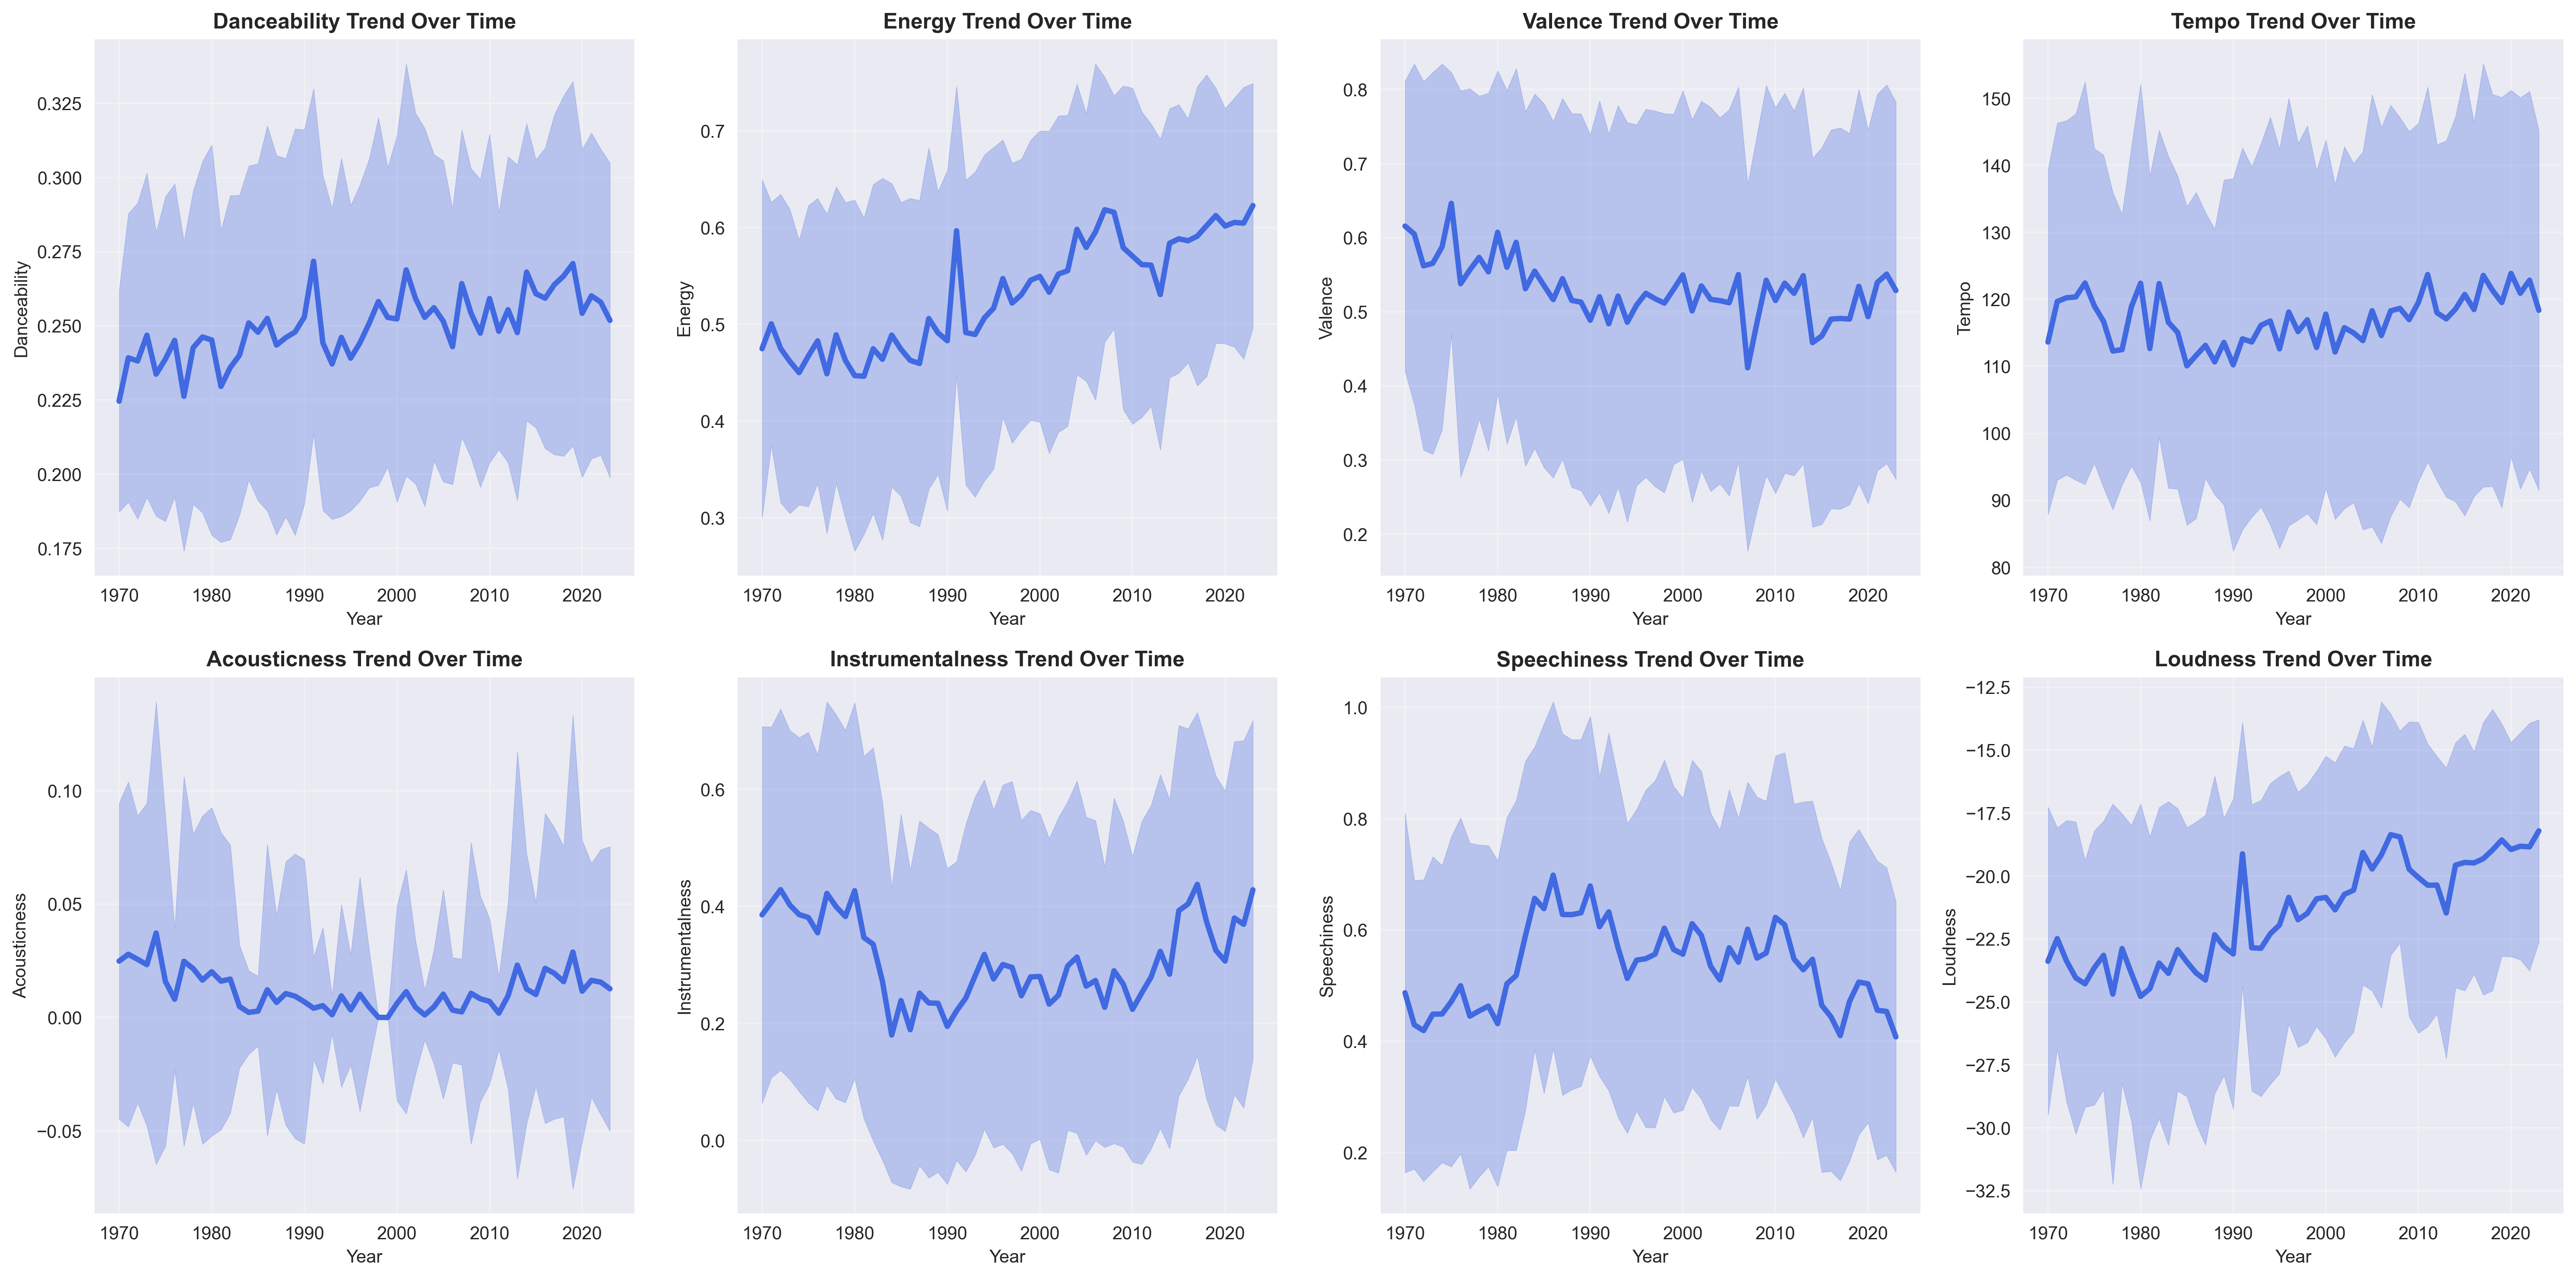
\includegraphics[width=\linewidth]{figures/audio_feature_trends.png}
      \caption{Annual means ($\pm$1 s.d.) for all 8 \texttt{librosa} features. Directional trends are strong and consistent: \textbf{loudness, energy, and speechiness rise} monotonically; \textbf{acousticness falls}. Instrumentalness is near-zero throughout (vocals dominate). Valence shows no clear trend.}
    \end{figure}
  \end{block}

\end{column}

\separatorcolumn

% ====================
% COLUMN 2
% ====================
\begin{column}{\colwidth}

  \begin{block}{Sonic Convergence: PCA \& Convex Hulls}

    \begin{figure}
      \centering
      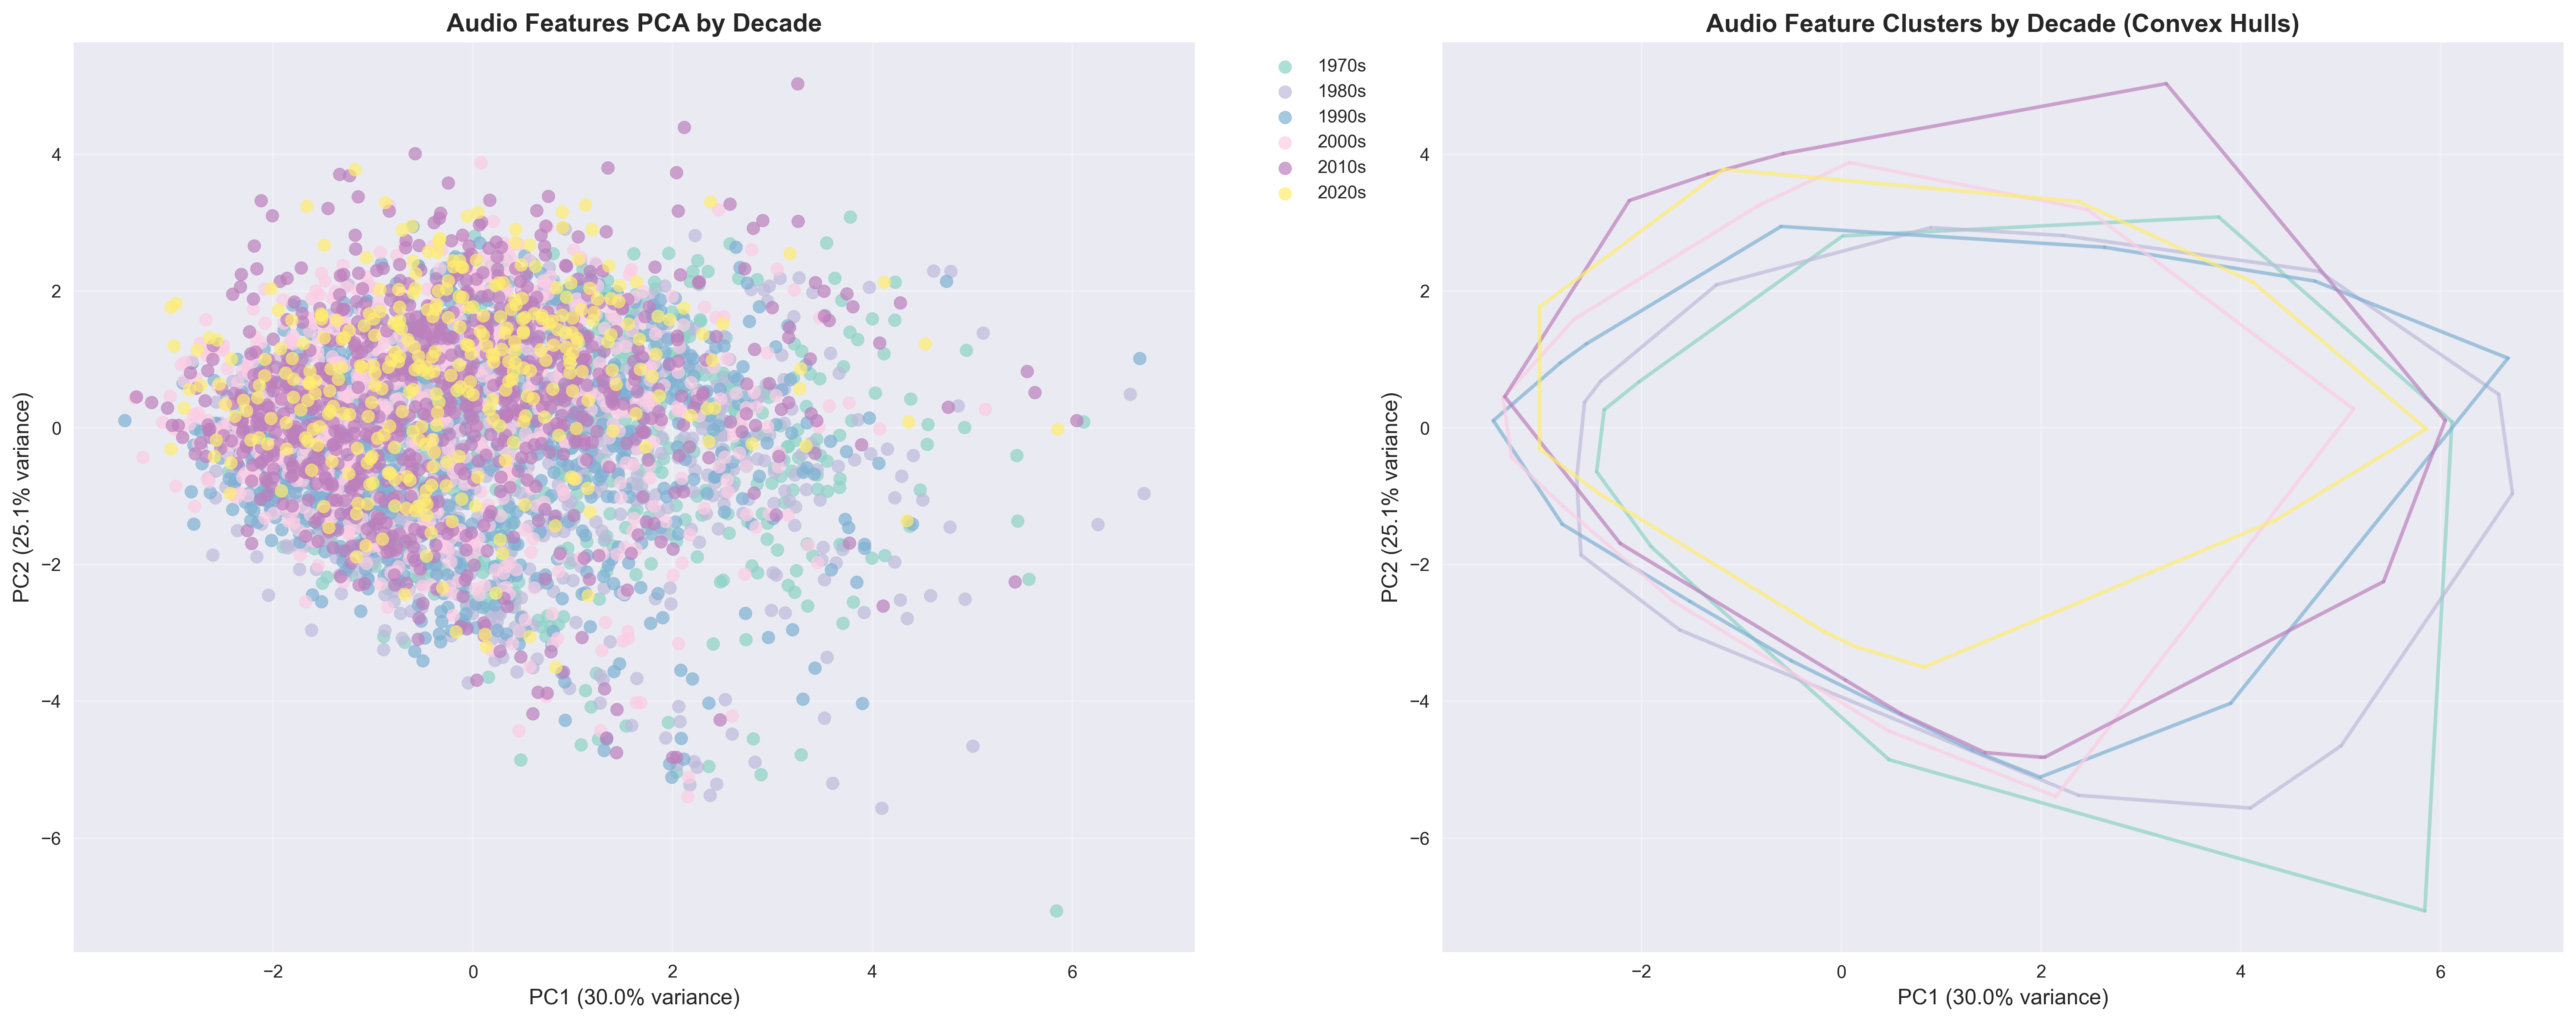
\includegraphics[width=\linewidth]{figures/audio_pca_analysis.png}
      \caption{PCA of all 8 audio features per decade (scatter + convex hulls). The hull enclosing each decade's point cloud is the primary convergence metric: a shrinking hull means hits are occupying a smaller region of sonic space.}
    \end{figure}

    \begin{center}
      \begin{tabular}{lcc}
        \toprule
        Decade & Hull Area & Change \\
        \midrule
        1970s & 59.9 & --- \\
        1980s & 57.8 & $-3.5\%$ \\
        1990s & 51.4 & $-11.1\%$ \\
        2000s & 47.3 & $-8.0\%$ \\
        2010s & 60.8 & $+28.5\%$ \\
        2020s & \textbf{41.9} & $-31.1\%$ \\
        \bottomrule
      \end{tabular}
    \end{center}

    The pattern is non-monotonic but ultimately convergent. Gradual sonic narrowing from the 1970s through the 2000s ($-21\%$ total) is interrupted by a 2010s expansion --- streaming opened the charts to more genres simultaneously --- before the 2020s collapse to the all-time minimum. The 2020s hull is \textbf{30\% smaller} than the 1970s despite covering only four years of data.

  \end{block}

  \begin{block}{Cosine Similarity Between Decade Centroids}

    \begin{figure}
      \centering
      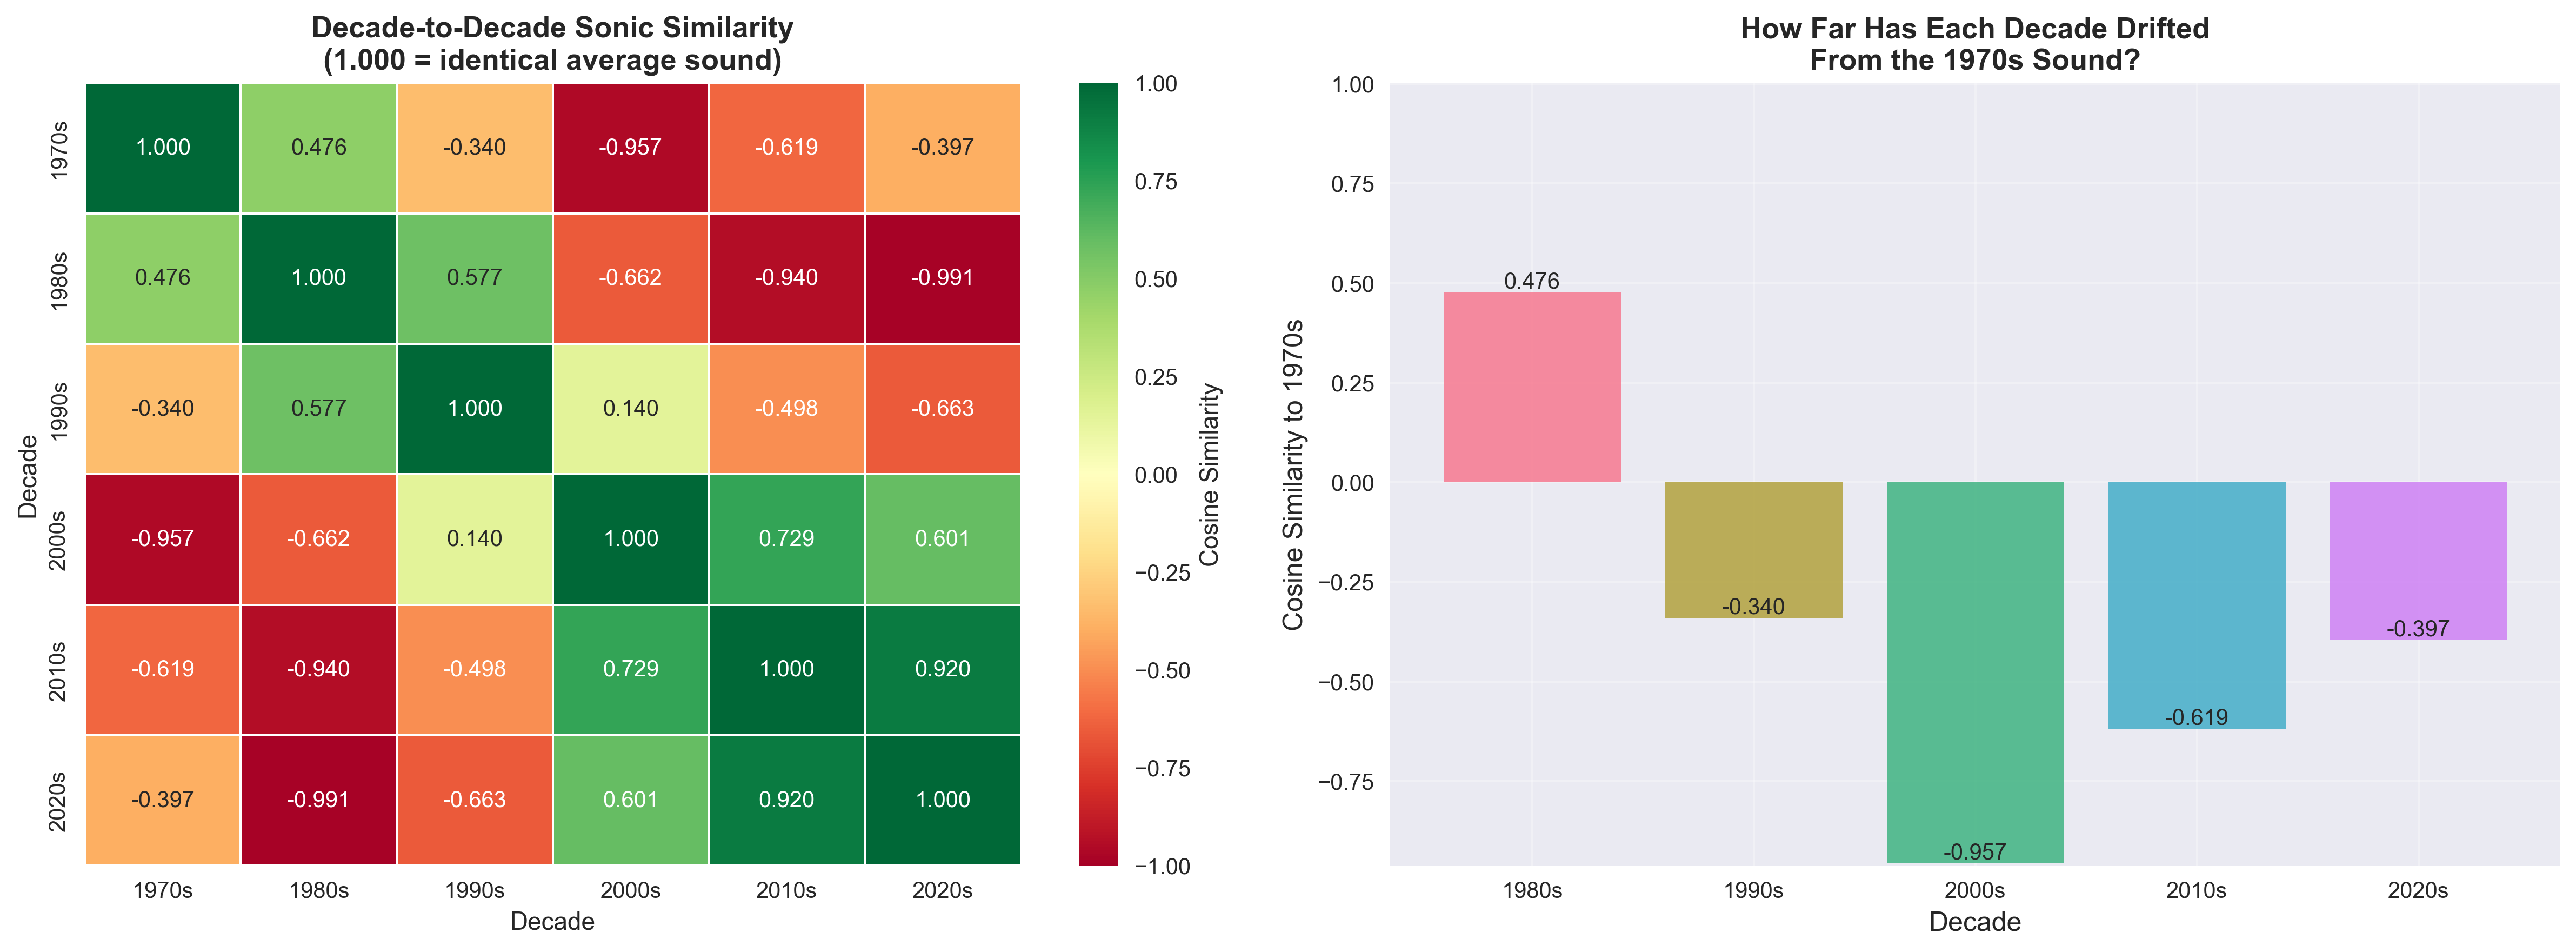
\includegraphics[width=\linewidth]{figures/decade_similarity_heatmap.png}
      \caption{Cosine similarity of per-decade audio centroids (StandardScaler-normalized). Values near $+1$ = decades point the same direction in feature space; near $-1$ = acoustically opposite.}
    \end{figure}

    The heatmap reveals a fundamental structural reversal across the 50-year span:

    \begin{itemize}
      \item \textbf{1980s $\leftrightarrow$ 2020s: $r = -0.99$} (near-perfectly opposite). The 1980s era featured moderate loudness ($-23.6$ dB), high acousticness, and minimal speechiness. The 2020s invert all three: loudness reached $-18.7$ dB, acousticness collapsed, and rap/trap drove speechiness to its peak.
      \item \textbf{2010s $\leftrightarrow$ 2020s: $r = +0.92$} (near-identical). Streaming locked in a sonic template that persists into the current decade.
      \item \textbf{1990s is the hinge decade}: the only era without a strongly negative cosine partner, sitting at the inflection point between pre- and post-digital production aesthetics.
    \end{itemize}

  \end{block}

  \begin{block}{Decade Classification (Convergence Test)}

    \begin{center}
      \begin{tabular}{lccc}
        \toprule
        Model & Accuracy & Macro F1 & vs.\ Baseline \\
        \midrule
        Random Forest       & 34.1\% & 0.29 & $+2.0\times$ \\
        Logistic Regression & 32.2\% & 0.30 & $+1.9\times$ \\
        KNN ($k{=}7$)       & 26.3\% & 0.23 & $+1.6\times$ \\
        \midrule
        Random baseline     & 16.7\% & --- & --- \\
        \bottomrule
      \end{tabular}
    \end{center}

    \smallskip
    Models perform at 2$\times$ random chance but with heavily blurred boundaries: adjacent decades are the dominant confusion pattern. The 2020s are nearly never predicted correctly (class imbalance: 331 songs vs.\ $\sim$850 per other decade). SHAP analysis identifies \textbf{year} and \textbf{loudness} as the top predictors; audio features account for $\sim$55\% of discriminative power vs.\ $\sim$45\% for lyrics --- both channels carry real but insufficient signal to separate decades cleanly.

  \end{block}

\end{column}

\separatorcolumn

% ====================
% COLUMN 3
% ====================
\begin{column}{\colwidth}

  \begin{block}{Lyrical Convergence: Diversity, Repetition \& Sentiment}

    \begin{figure}
      \centering
      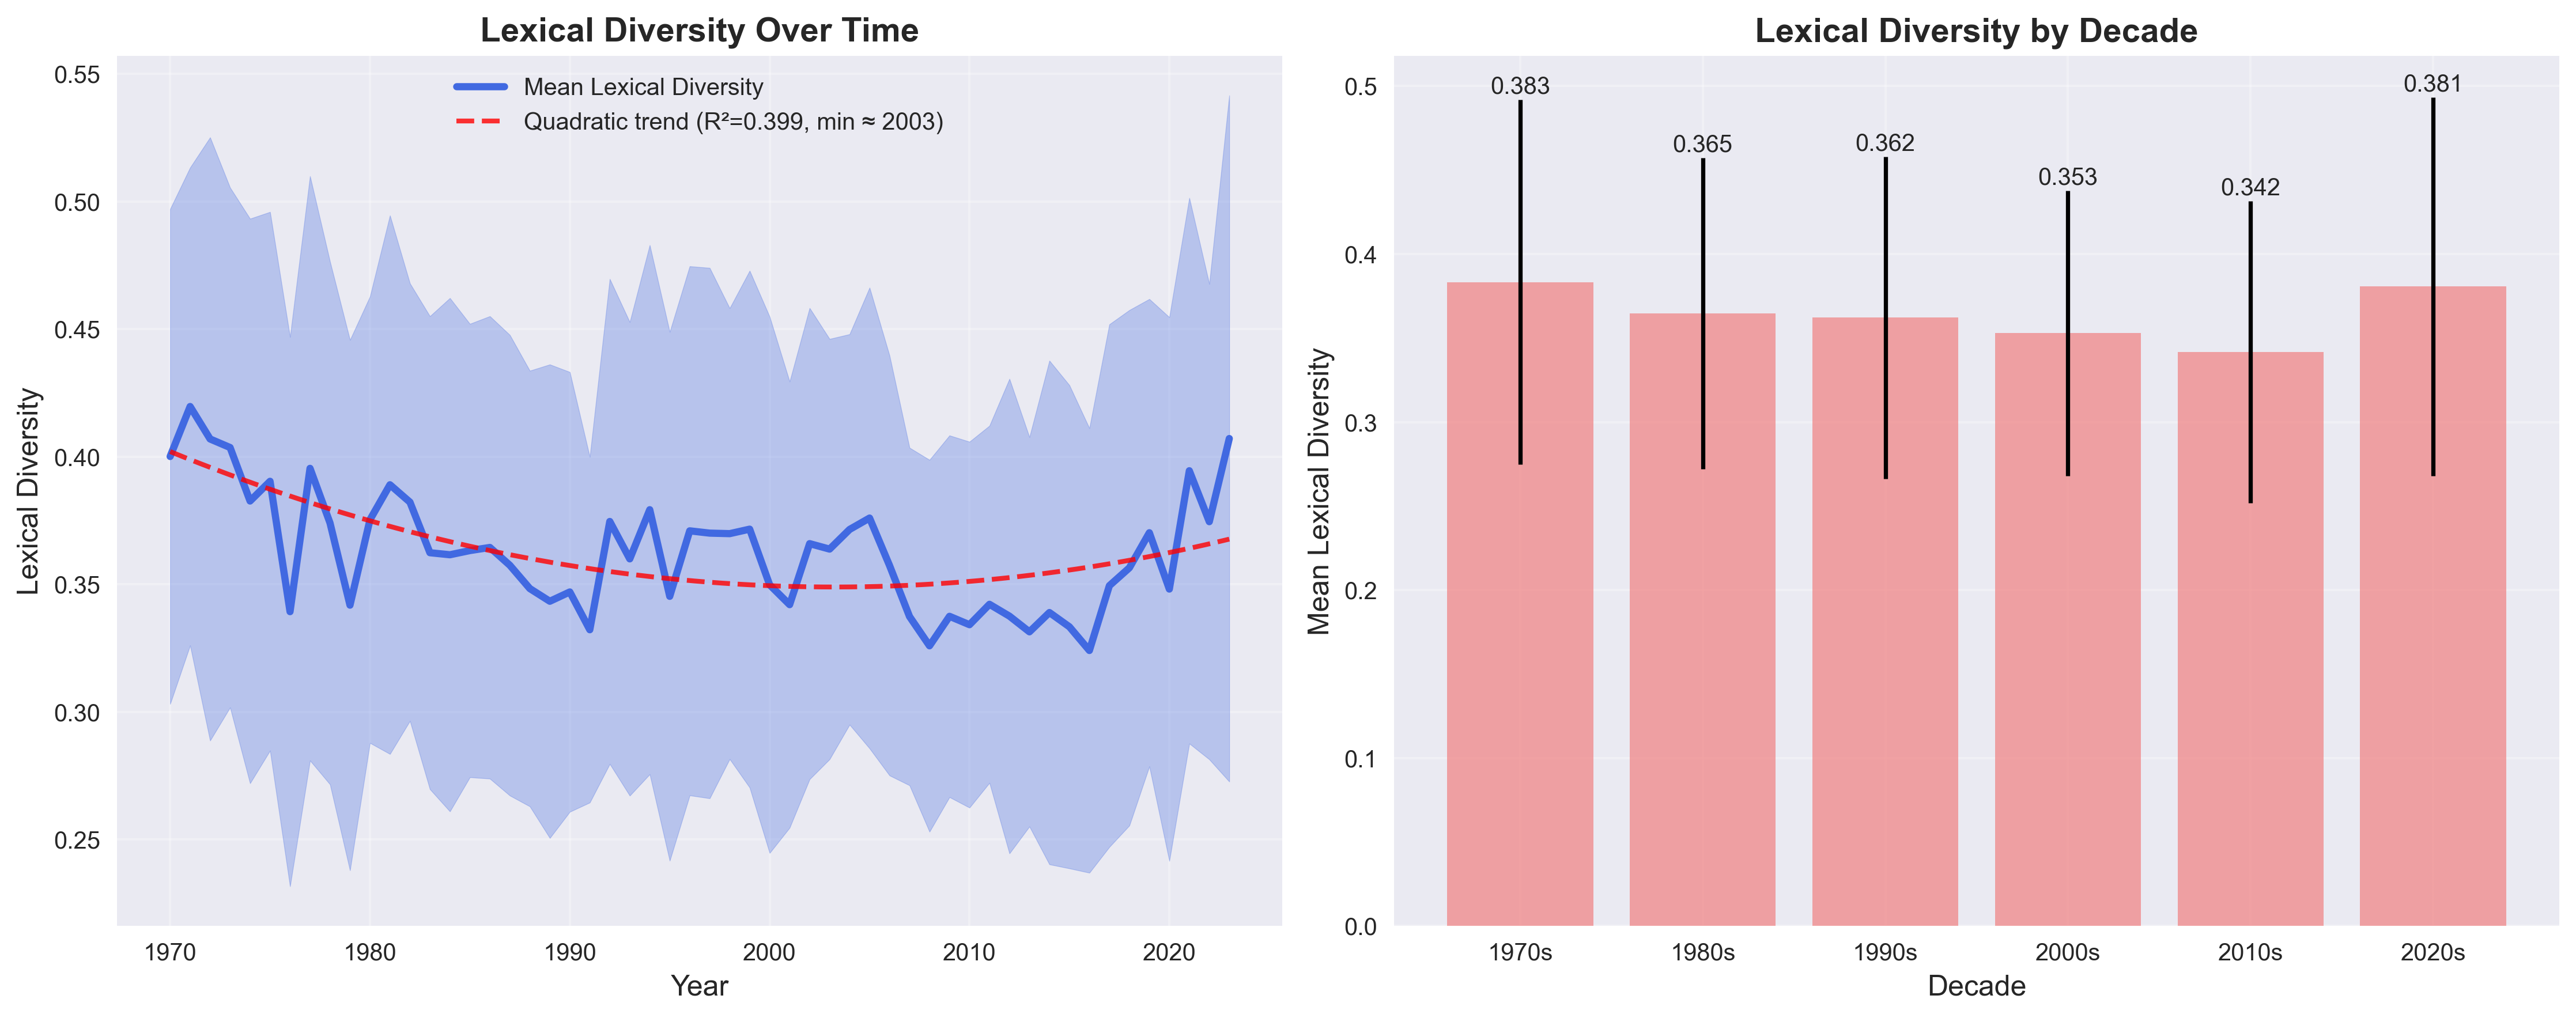
\includegraphics[width=\linewidth]{figures/lexical_diversity_analysis.png}
      \caption{Lexical diversity (unique/total words) 1970--2023 with quadratic trend ($R^2 = 0.68$, minimum $\approx$ 2007). The U-shape is statistically robust: Kruskal--Wallis $H = 99.89$, $p = 5.56 \times 10^{-20}$.}
    \end{figure}

    \textbf{Lexical Diversity} (unique/total words):

    \begin{center}
      \begin{tabular}{lcc}
        \toprule
        Decade & Mean Lex.\ Div. & Bonferroni vs.\ 1970s \\
        \midrule
        1970s & 0.383 & --- \\
        1980s & 0.365 & $p < 0.01$ \\
        1990s & 0.358 & $p < 0.001$ \\
        2000s & 0.353 & $p < 0.001$ \\
        2010s & 0.342 \textbf{(trough)} & $p < 0.001$ \\
        2020s & 0.381 & $p = 1.0$ (n.s.) \\
        \bottomrule
      \end{tabular}
    \end{center}

    The 2020s recovery to 0.381 is \textbf{not significantly different from the 1970s} --- lyrical vocabulary has returned to its starting point, though via a very different sonic backdrop.

    \smallskip
    \textbf{LZ77 Compressibility} captures \emph{structural} repetition (verse/chorus patterns, hook loops) independently of vocabulary size. The 2010s show a dramatic spike: compressibility = 0.848 vs.\ 0.77--0.79 in all other decades (1990s vs.\ 2010s: $p = 0.0003$, Cohen's $d = 0.89$, a large effect). The 2020s drop sharply to 0.750, below even the 1970s baseline --- suggesting not just vocabulary recovery but a structural loosening of song form.

    \smallskip
    \textbf{Sentiment} (TextBlob polarity) tells a split story. Across the full Hot 100, polarity declined monotonically from 0.165 (1970s) to 0.080 (2010s). But among \textbf{top-10 hits only}, the 2020s recover to 0.164 --- matching the 1970s. The biggest hits trend happier even as the broader chart darkens. Filtering to top-10 also collapses the lexical diversity U-shape to a flat line, suggesting vocabulary variation is driven by mid-chart songs rather than the very biggest hits.

  \end{block}

  \begin{block}{Discussion: Three Phases of Homogenization}

    Our findings support a convergence narrative, but one that unfolds in three structurally distinct phases shaped by industry technology:

    \smallskip
    \textbf{Phase 1 --- Gradual Narrowing (1970s--2000s):} Radio consolidation and the CD era progressively filtered the sonic and lyrical range of chart hits. Hull area fell 21\%; lexical diversity declined steadily. Production aesthetics began converging around a polished, louder template.

    \smallskip
    \textbf{Phase 2 --- Streaming Paradox (2010s):} Spotify and playlist culture allowed a wider range of genres to chart simultaneously, \emph{expanding} the PCA hull to its largest recorded size. Yet the algorithmic pressure to maximize replay value produced the most lyrically repetitive decade on record (LZ77 peak, lexical diversity trough). More sounds, less originality --- a form of sonic diversity masking lyrical homogenization.

    \smallskip
    \textbf{Phase 3 --- Diverging Channels (2020s):} TikTok-driven virality rewards narrative specificity and lyrical hooks, pulling vocabulary diversity back to 1970s levels and reducing structural repetition. Simultaneously, streaming-optimized production has never been more homogeneous (hull area 41.9, all-time minimum). The two channels are now moving in \emph{opposite} directions.

    \smallskip
    \textit{\textbf{Caveat:} 2020s data covers only 2020--2023 (331 songs vs.\ $\sim$850 per other decade). The reversal is statistically significant but may shift as the decade completes.}

  \end{block}

  \begin{block}{References}
    \footnotesize{
    \begin{enumerate}
      \item Billboard Hot 100 data via \textit{billboard.py}.
      \item McFee et al.\ ``librosa: Audio and Music Signal Analysis in Python.'' \textit{SciPy Conf.}, 2015.
      \item \label{interiano2018} Interiano et al.\ ``Musical trends and predictability of success in contemporary songs.'' \textit{Royal Society Open Science}, 2018.
      \item Serra et al.\ ``Measuring the Evolution of Contemporary Western Popular Music.'' \textit{Scientific Reports}, 2012.
      \item Lundberg \& Lee. ``A Unified Approach to Interpreting Model Predictions (SHAP).'' \textit{NeurIPS}, 2017.
    \end{enumerate}
    }
  \end{block}

\end{column}

\separatorcolumn
\end{columns}
\end{frame}

\end{document}
